El problema de los puntos más cercanos ({\em Closest Pair Problem}) parte de un conjunto de {\em n} puntos pertenecientes al plano XY, donde cada punto está representado por sus coordenadas {\em X} y {\em Y}, se desea hallar encontrar el par de puntos tal que la distancia entre ambos puntos es mínima. El algoritmo debe devolver dichos puntos o la distancia .

\begin{figure}[h]
	\centering 
	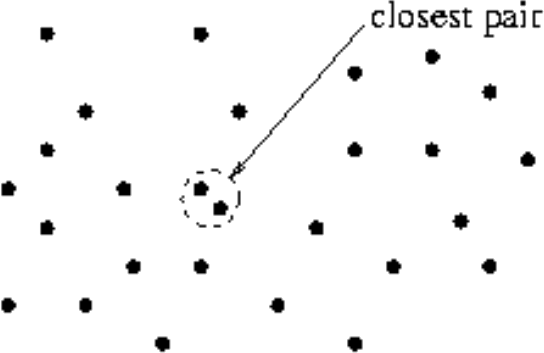
\includegraphics[scale=0.3]{img/closest_pair}
	\label{contexto:figura1}
\end{figure}